\documentclass{standalone}
\begin{document}
\subsection{Prediction of Response}

The accuracy for the prediction of response was measured by using different metrics.
\\
In Table \ref{tab:classreport} you can see the classification report made by the Precision, Recall, and F1 score for each class (Class 0 for complete response and Class 1 for moderate response).
\\
Unfortunately, the TRG value was missing for some patients, therefore some of them were excluded from the analysis.
In the end, the total number of patients was 32, that is the sum of the \textit{support} column values for Class 0 and Class 1.
\\
The classifier model was cross-validated to avoid the presence of \textit{bias} during the split into training and test set of the data on 500 simulations, evaluating the Matthews Correlation coefficient (MCC).
The result is a distribution of the MCC, that you can see in Figure \ref{MCC}, with a median $MCC=0.55$ .

\begin{table}[ht]
	\centering
	\begin{tabular}{ccccc}
		\toprule
		  & \textbf{Precision}  & \textbf{Recall} & \textbf{F1-Score} & \textbf{Support}\\
	    \midrule
		\textbf{Class 0} &  0.71 &  0.77 &  0.74 &  13\\
	    \midrule
		\textbf{Class 1} &  0.83 &  0.79 &  0.81 &  19\\
		\bottomrule
	\end{tabular}
	\caption{Classification report}
	\label{tab:classreport}
\end{table}



\begin{figure}[ht]

	\centering
	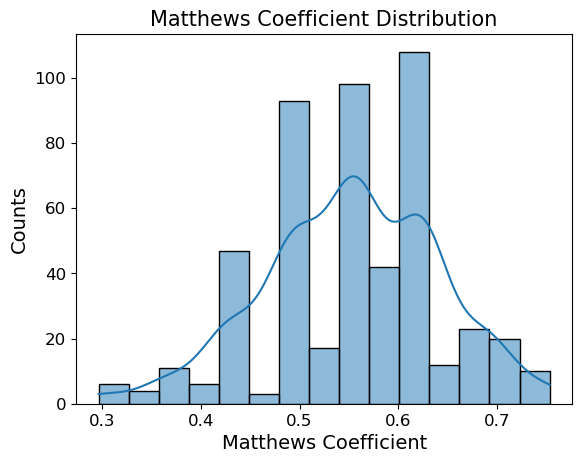
\includegraphics[width=0.65\textwidth]{../images/MCC.png}

	\caption{Matthews Correlation coefficient distribution for the pipeline obtained after 500 simulations.}
	\label{MCC}
	
	\end{figure}


\newpage
I also computed the confusion matrix , in Figure \ref{confmatrix}, to evaluate the accuracy of the classification.
For Class 0, so for a complete response, the well-classified instances are 10 over a total of 13, thus the wrong-classified ones are 3.
For Class 1, so for a moderate response, the well-classified instances are 15 over a total of 19, thus the wrong-classified ones are 4.


\begin{figure}[htp]

    \centering
    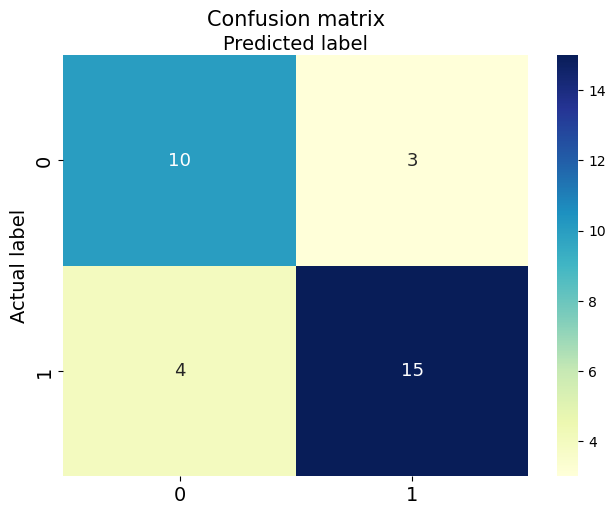
\includegraphics[width=0.8\textwidth]{../images/confmatrix.png}

    \caption{Confusion Matrix. The rows of the matrix represents the instances in an actual class while each column represents the instances in a predicted class. Class 0 means a complete response while Class 1 a moderate one. }
    \label{confmatrix}
    
\end{figure}

The diagnostic ability of the classifier was also measured by computing the Receiver Operating Characteristic curve, or ROC curve, in Figure \ref{ROC}.
As you can see, the AUC for both the classes is 0.82.
I computed the average curve for Class 0 and Class 1, both by taking into account class imbalance (micro-average) and by giving the same weight to the classes (macro-average). 

\begin{figure}[htp]

    \centering
    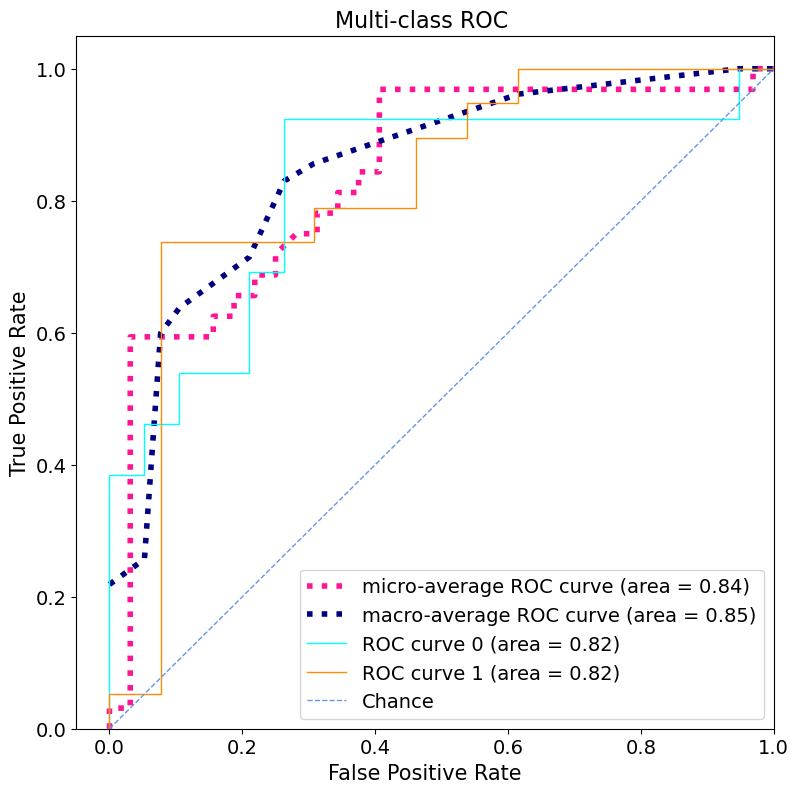
\includegraphics[width=0.8\textwidth]{../images/ROC.png}

    \caption{Receiver Operating Characteristic curve, or ROC curve.
	Class 0 indicates a complete response to chemo-radiotherapy while Class 1 a moderate one.
	The average curve for Class 0 and Class 1, is computed both by taking into account class imbalance (micro-average) and also by giving the same weight to the classes (macro-average).}
    \label{ROC}
    
\end{figure}

\end{document}